% SVN info for this file
\svnidlong
{$HeadURL$}
{$LastChangedDate$}
{$LastChangedRevision$}
{$LastChangedBy$}

\chapter{Alla ricerca della lunghezza dell'ellisse}
\labelChapter{ellipseintroduction}

\begin{introduction}
‘‘BEEP BOOP QUESTA È UNA CITAZIONE.''
\begin{flushright}
	\textsc{Marinobot,} dopo aver finito le citazioni stupide.
\end{flushright}
\end{introduction}
\lettrine[findent=1pt, nindent=0pt]{U}{na circonferenza} e un'\emph{ellisse} a primo acchito possono sembrare molto simili: in fondo, una circonferenza non è altro che un'ellisse i cui punti focali coincidono e dunque l'ellisse si può vedere come una circonferenza ‘‘allungata'' rispetto ad un asse. Il valore dell'area delimitata da una circonferenza ($\pi r^2$) e la lunghezza di una circonferenza ($2\pi r$) sono ben noti già dall'antichità, i cui calcoli sono stati opportunamente formalizzati in epoca moderna; tuttavia, riguardo l'ellisse, ci accorgiamo di aver incontrato nel corso degli studi precedenti quasi esclusivamente il valore dell'area delimitata da essa ($\pi ab$), ma \emph{non la lunghezza dell'ellisse}. Come mai?\\
\section{Una domanda banale: la lunghezza di un'ellisse}
Partiamo col seguente \textit{quiz}: quale delle seguenti tre espressioni è il valore, o una sua \textit{approssimazione}, della lunghezza di un'ellisse di semiassi di lunghezza $a$ e $b$?
\begin{enumerate}[label=\alph*)]
	\item $L\left(a,b\right)=\pi ab$
	\item $L\left(a,b\right)\approx \pi \left(a+b\right)+3\pi\frac{\left(a-b\right)^2}{10\left(a+b\right)+\sqrt{a^2+14ab+b^2}}$
	\item $L\left(a,b\right)\approx 2\pi a$.
\end{enumerate}
Chiaramente, come abbiamo detto nell'introduzione del capitolo, la lunghezza dell'ellisse \textit{non} è una formula nota dagli studi passati e possiamo (per ora) solamente escludere la \textit{prima risposta}, in quanto essa è il valore dell'\textbf{area} delimitata dell'ellisse.
\begin{observe}
	  Possiamo escludere la prima risposta anche per motivi puramente \textbf{dimensionali}: $a$ e $b$ sono, dimensionalmente parlando, due lunghezze, quindi $\pi ab$ deve essere una \textit{lunghezza al quadrato}, cioè un'area e non può essere una lunghezza!
\end{observe}
In realtà, la domanda del quiz è mal posta: le risposte \textit{b)} e \textit{c)} sono entrambe corrette.\\
Il matematico indiano Srinivasa Aiyangar Ramanujan fornì come nota a margine non commentata in un suo articolo del 1914 (\cite{ramanujan:1914piapprox}) l'approssimazione \textit{b)}:
\begin{equation*}
	L\left(a,b\right)\approx \pi\left(\left(a+b\right)+3\frac{\left(a-b\right)^2}{10\left(a+b\right)+\sqrt{a^2+14ab+b^2}}\right)
\end{equation*}
Vedremo fra poco che anche l'approssimazione data dalla \textit{a)} è anch'essa lecita.\\
Il motivo per cui diamo approssimazioni ma non formule esatte per la lunghezza dell'ellisse è dovuto al fatto che \textit{non esiste} una formula esplicita in termini di \textit{funzioni elementari}, bensì possiamo esprimerla soltanto come \textbf{somma di una serie}.
\begin{theorema}[Lunghezza dell'ellisse di semiassi di lunghezza $a$ e $b$.]~{}\\
	Siano $a\geq b$ le lunghezze dei semiassi dell'ellisse e $e=e\left(a,b\right)=\frac{\sqrt{a^2-b^2}}{a}\in\left[0,1\right)$ l'\textbf{eccentricità}\index{eccentricità}; allora si ha
	\begin{equation}
		L\left(a,b\right)=2\pi a\sum_{j=0}^{+\infty}\frac{1}{1-2j}\left(\frac{\left(2j-1\right)!!}{\left(2j\right)!!}e^j\right)^2
	\end{equation}
dove $!!$ indica il \textbf{doppio fattoriale}\index{fattoriale!doppio}:
\begin{itemize}
	\item $\left(-1\right)!!=0!!=1$
	\item $\forall n\in\naturalset\quad n!!=\begin{cases}
		n\cdot \left(n-2\right)\cdot \ldots \cdot 6 \cdot 4 \cdot 4 \cdot 2\text{ se }n>0\text{ è pari}\\
		n\cdot \left(n-2\right)\cdot \ldots \cdot 5 \cdot 3 \cdot 2 \cdot 1\text{ se }n>0\text{ è dispari}\\
	\end{cases}$
\end{itemize}
\end{theorema}
Il primo termine della serie fornisce l'approssimazione espressa nella risposta \textit{a)}:
\begin{equation*}
	L\left(a,b\right)\approx 2\pi a
\end{equation*}
\subsection{La problematica dimostrazione della lunghezza dell'ellisse: la serie di Taylor}
\begin{minipage}{0.49\textwidth}
	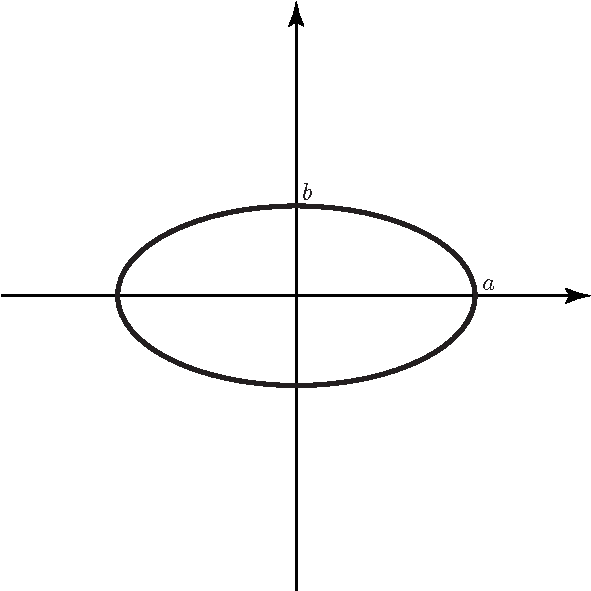
\includegraphics[trim=0cm 2.25cm 0cm 0cm, clip, scale=0.65]{images/ellisse.pdf}
\end{minipage}\hspace{-2mm}
\begin{minipage}{0.50\textwidth}
Dimostriamo finalmente la lunghezza dell'ellisse. Come è noto dal corso di \textsc{Analisi 2}, per una curva \textit{regolare} come l'ellisse è possibile calcolarne la lunghezza usando un'opportuna parametrizzazione.\\
Poniamo $a\geq b$ le lunghezze dei semiassi ed $e=\frac{\sqrt{a^2-b^2}}{a}\in\left[0,1\right)$ l'eccentricità. Una parametrizzazione è
\begin{equation*}
	\vec{r}\left(t\right)=\left(a\sin t,\ b\cos t\right)\quad t\in\left[0, 2\pi\right]
\end{equation*}
\end{minipage}\\
Allora
\begin{align*}
		L&=\int_{0}^{2\pi}\norm{\vec{r}'\left(t\right)}dt=\int_{0}^{2\pi}\norm{\left(a\cos t,\ -b\sin t\right)}dt=\int_{0}^{2\pi}\sqrt{a^2\cos^2t+b^2\sin^2t}dt=\\
		&=\int_{0}^{2\pi}\sqrt{a^2-\left(a^2+b^2\right)\sin^2t}dt=a\int_{0}^{2\pi}\sqrt{1-e^2\sin^2t}
\end{align*}
C'è un problema: la funzione $f\left(t\right)=\sqrt{1-e^2\sin^2t}$ non è \textbf{elementarmente integrabile}, cioè non ammette primitive in termini di funzioni elementari.
\begin{attention}
	Non essere elementarmente integrabile \textit{non} significa che non sia integrabile! La funzione integranda $f\left(t\right)$ è continua su $\left[0, 2\pi\right]$, dunque per il \textit{teorema fondamentale del calcolo integrale} ammette primitive su $\left[0, 2\pi\right]$. Una di esse è
	\begin{equation*}
		F\left(t\right)=\int_{0}^{t}\sqrt{1-e^2\sin^2y}dy\quad\forall y\in\left[0,2\pi\right]
	\end{equation*}
	Il problema è che \textit{non} possiamo riscrivere $F$ in modo esplicito usando \textit{solo} funzioni elementari.
\end{attention}
Questo tipo di integrale è detto \textbf{integrale ellittico}\index{integrale!ellittico}.
\begin{digression}
	Gli \textit{integrali ellittici} si incontrano in molti ambiti matematici. Ad esempio, appaiono nella risoluzione dell'equazione differenziale del moto di un pendolo semplice:
	\begin{equation*}
		\ddot{\theta}=-\frac{g}{l}\sin\theta
	\end{equation*}
	Sono il motivo per cui tale equazione si studia spesso per piccole oscillazioni, in modo da poter operare una linearizzazione $\sin\theta\sim\theta$ e calcolare il moto senza passare per tali integrali non calcolabili.\\
	Un altro esempio della loro importanza è noto agli appassionati di \textsc{Geometria}: infatti, la branca della Geometria Algebrica nasce anche dagli studi su tali integrali.
\end{digression}
Potremmo limitarci a considerare l'intero integrale ellittico come una nuova funzione, ma al più potremmo calcolarne il valore tramite metodi dell'\textsc{Analisi Numerica}. Invece, proviamo a riscrivere l'integrale utilizzando uno \textbf{sviluppo in serie} della funzione integranda.\\
Poniamo $x=-e^2\sin^2t$ e osserviamo che
\begin{equation*}
	\sqrt{1-e^2\sin^2 t}=\sqrt{1+x}=\left(1+x\right)^{\nicefrac{1}{2}}=\left(1+x\right)^\alpha\quad\text{dove }\alpha=\frac{1}{2}
\end{equation*}
Poichè $\left(1+x\right)^\alpha$ è una funzione di classe $\mathcal{C}^\infty$ in un intorno di $x=0$, si può approssimare localmente col \textbf{polinomio di Taylor}\index{polinomio di Taylor} di ordine $n$ centrato in $x=0$, $\forall n\geq 0$. Se il polinomio in questione è
\begin{equation*}
	P_{n,0}\left(x\right)=\sum_{j=0}^{n}\binom{\alpha}{j}x^j\quad\forall n\geq 0
\end{equation*}
con $\displaystyle\binom{\alpha}{j}$ il \textbf{coefficiente binomiale generalizzato}\index{coefficiente binomiale!generalizzato}\footnote{Nelle ‘‘Note aggiuntive'', a pagina \pageref{coefficientebinomialgeneralizzato} è possibile trovare la definizione e le proprietà del binomiale generalizzato.}, allora l'approssimazione dell'integranda data dal polinomio di Taylor è proprio
\begin{equation*}
	\left(1+x\right)^{\nicefrac{1}{2}}\approx\sum_{j=0}^{n}\binom{\nicefrac{1}{2}}{j}x^j\quad\forall n\geq 0
\end{equation*}
Risostituendo $x=-e^2\sin^2t$ abbiamo un'approssimazione dell'integranda. Tuttavia, noi vorremmo un \textit{risultato esatto}.\\
Sappiamo intuitivamente che più termini si hanno nello sviluppo di Taylor, più accurata è l'approssimazione; cosa succede per $n\to\infty$? Dobbiamo studiare la somma di serie
\begin{equation*}
	\sum_{j=0}^{+\infty}\binom{\nicefrac{1}{2}}{j}x^j
\end{equation*}
Già ci dobbiamo porre nuove domande: la serie \textit{converge} e per quali valori di $x$? Supponendo che la serie converga per opportuni valori di $x$, la serie converge proprio a $\left(1+x\right)^{\nicefrac{1}{2}}$?\\
\textit{In generale}, per $f\in\mathcal{C}^\infty$ qualsiasi \textbf{NO}, la serie di Taylor non converge proprio e se converge non converge ad $f$! Tuttavia, in questo caso siamo particolarmente fortunati: $\forall x\in \left(-1, 1\right)$ la serie converge\footnote{Nelle ‘‘Note aggiuntive'', a pagina XXX è possibile trovare la dimostrazione di tale convergenza.} e vale
\begin{equation*}
	\left(1+x\right)^{\frac{1}{2}}=\sum_{j=0}^{+\infty}\binom{\nicefrac{1}{2}}{j}x^j\quad\forall n\geq 0\quad \forall x\in\left(-1, 1\right)
\end{equation*}
In questa prima parte della dimostrazione abbiamo capito che è importante determinare quando è possibile passare dalla semplice \textit{approssimazione} di una funzione con il \textit{polinomio di Taylor} a poter riscrivere una funzione come una \textbf{serie di Taylor}\index{serie di Taylor} di funzioni opportune.
\subsection{La problematica dimostrazione della lunghezza dell'ellisse: passaggio al limite sotto segno di integrale}
Torniamo al problema originale. Ricordando che $x=-e^2\sin^2 t$, poiché $t\in\left[0,2\pi\right]$ si ha che $x\in\left[-e^2, 0\right]\subseteq\left(-1, 1\right)$ dato che $e^2<1$. Possiamo riscrivere l'integranda come il suo sviluppo in \textit{serie di Taylor}:
\begin{align*}
	\left(1-e^2\sin^2t\right)^{\nicefrac{1}{2}}=\sum_{j=0}^{+\infty}\binom{\nicefrac{1}{2}}{j}\left(-e^2\sin^2t\right)^j=\sum_{j=0}^{+\infty}\binom{\nicefrac{1}{2}}{j}\left(-1\right)^je^{2j}\sin^{2j}t\quad \forall t\in\left[0, 2\pi\right]
\end{align*}
Sostituiamo nell'integrale; poiché la funzione è pari e simmetrica, possiamo ricondurci a studiare l'integrale su $\left[0,\nicefrac{\pi}{2}\right]$:
\begin{equation*}
L=a\int_{0}^{2\pi}\left(1-e^2\sin^2t\right)^{\nicefrac{1}{2}}dt=4a\int_{0}^{\frac{\pi}{2}}\left(1-e^2\sin^2t\right)^{\nicefrac{1}{2}}dt=4a\int_{0}^{\frac{\pi}{2}}\sum_{j=0}^{+\infty}\binom{\nicefrac{1}{2}}{j}\left(-1\right)^je^{2j}\sin^{2j}tdt\squarequal
\end{equation*}
Incontriamo un nuovo problema: cos'è l'\textbf{integrale di una serie}? Se avessimo una somma di un numero \textit{finito} di termini per la \textit{linearità} dell'integrale potremmo scambiare la sommatoria con l'integrale, ma è possibile farlo nel caso di una serie?\\
Riscriviamo l'espressione precedente con la definizione di serie come \textit{limite} per $n\to +\infty$ delle \textit{ridotte}:
\begin{equation*}
	\squarequal 4a\int_{0}^{\frac{\pi}{2}}\lim_{n\to +\infty}\left(\sum_{j=0}^{n}\binom{\nicefrac{1}{2}}{j}\left(-1\right)^je^{2j}\sin^{2j}t\right)dt
\end{equation*}
Il problema precedente si può riformulare come \emph{‘‘È possibile scambiare integrale e limite?''}. Tale questione è come il problema del \textbf{passaggio al limite sotto segno di integrale}.\\
\textit{In generale}, la risposta è \textbf{NO}: non è possibile scambiare limite e integrale. Ciò nonostante anche questa volta siamo particolarmente fortunati e il passaggio è \textit{lecito}\footnote{Nelle ‘‘Note aggiuntive'', a pagina XXX è possibile trovare la dimostrazione che in questo caso il passaggio è lecito.} e si ha
\begin{align*}
	L&=4a\lim_{n\to +\infty}\int_{0}^{\frac{\pi}{2}}\sum_{j=0}^{n}\binom{\nicefrac{1}{2}}{j}\left(-1\right)^je^{2j}\sin^{2j}tdt\\
	&=4a\lim_{n\to +\infty}\sum_{j=0}^{n}\int_{0}^{\frac{\pi}{2}}\binom{\nicefrac{1}{2}}{j}\left(-1\right)^je^{2j}\sin^{2j}tdt\\
	&=4a\sum_{j=0}^{+\infty}\binom{\nicefrac{1}{2}}{j}\left(-1\right)^je^{2j}\int_{0}^{\frac{\pi}{2}}\sin^{2j}tdt
\end{align*}
Completando il calcolo dell'integrale\footnote{Nelle ‘‘Note aggiuntive'', a pagina XXX è possibile trovare tale calcolo.} si ottiene la formula della lunghezza scritta precedentemente.\\
\section{Non banali conseguenze di una domanda banale}
Abbiamo finalmente raggiunto una \textit{risposta}, seppur assolutamente non banale, alla domanda che ci eravamo posti originalmente: qual è la \textit{lunghezza dell'ellisse}? Nel far ciò ci siamo imbattuti in tutta una serie di problemi: esplicitare integrali non \textit{elementarmente} risolvibili, la \textit{convergenza} di \textit{serie di Taylor} di funzioni ad una funzione specifica, il \textit{passaggio al limite} sotto segno di \textit{integrale}.
La teoria matematica che tratteremo a partire dai capitoli successivi \textit{nasce} proprio da questi problemi apparsi nell'\textit{insidiosa ricerca} di una formula della lunghezza dell'ellisse.\\
In particolare, per capire quando era possibile il passaggio al limite sotto segno di integrale sono stati sviluppati diversi \textit{teoremi}, più o meno vantaggiosi da utilizzare, le cui ipotesi variano sensibilmente fra di loro: alcuni si inseriscono nella già nota \textit{teoria Riemanniana degli integrali}, mentre altri richiedono ipotesi completamente diverse. È da questi innumerevoli approcci al problema che, storicamente parlando, fu tale quesito a dare un \textit{impeto} fondamentale allo sviluppo della \textbf{teoria degli integrali di Lebesgue}.